\documentclass{beamer}
\usepackage[utf8]{inputenc}
\usepackage{graphicx}
\usepackage{subcaption}
\usepackage{hyperref}


\setbeamertemplate{caption}[numbered]


\title[Microservices and Monolithic Solutions]{
	{\small Master's thesis}\\
	Microservices and Monolithic Solutions in the Web Applications
}

\author[Krystian Skibiński]{Krystian Skibiński
}


\usetheme{CambridgeUS}
\usecolortheme{orchid}


\makeatletter
\newcommand\titlegraphicii[1]{\def\inserttitlegraphicii{#1}}
\titlegraphicii{}
\setbeamertemplate{title page}
{
  \vbox{}
   {\usebeamercolor[fg]{titlegraphic}\inserttitlegraphic\hfill\inserttitlegraphicii\par}
  \begin{centering}
    \begin{beamercolorbox}[sep=8pt,center]{institute}
      \usebeamerfont{institute}\insertinstitute
    \end{beamercolorbox}
    \begin{beamercolorbox}[sep=8pt,center]{title}
      \usebeamerfont{title}\inserttitle\par%
      \ifx\insertsubtitle\@empty%
      \else%
        \vskip0.25em%
        {\usebeamerfont{subtitle}\usebeamercolor[fg]{subtitle}\insertsubtitle\par}%
      \fi%     
    \end{beamercolorbox}%
    \vskip1em\par
    \begin{beamercolorbox}[sep=8pt,center]{date}
      Zielona Góra, \usebeamerfont{date}\insertdate
    \end{beamercolorbox}%\vskip0.5em
    \begin{beamercolorbox}[sep=8pt,center]{author}
      \usebeamerfont{author}\insertauthor
    \end{beamercolorbox}
  \end{centering}
  %\vfill
}
\makeatother
\date{\today}

\begin{document}


	\section{Introduction}
	\begin{frame}[plain]
		\maketitle	
	\end{frame}
	
	\begin{frame}{Introduction}{}
		\textbf{Master thesis progress:}\\
		Done. Approved by the supervisor \checkmark \\
		~\\
		~\\
		\textbf{Table of contents:}
		\tableofcontents[sections={1-2}]
			\framebreak
		\tableofcontents[sections={3}]
	\end{frame}
	
	\subsection{Abstract}
	\begin{frame}{Abstract}
	The thesis concerns on comparison of two popular approaches, microservices and monolithic, used in creating websites. Its purpose is to show the similarities and differences between these patterns, as well as their properties and to indicate cases for which the given architecture works best. For its needs, two websites were created using these approaches.
	\end{frame}

	
	\section{Theoretical part}
	\subsection{What is a Web Application?}
	\begin{frame}{Web Applications}
		\textbf{Web applications} are computer programs, that use the browser as~a \textit{client}, which is used to provide and receive the data. Anther computer in that case called \textit{server} is storing that provided by user data and if they are needed, share them. \\
	
		\begin{figure}[h!]
  			\centering
  			\begin{subfigure}[b]{0.3\linewidth}
    			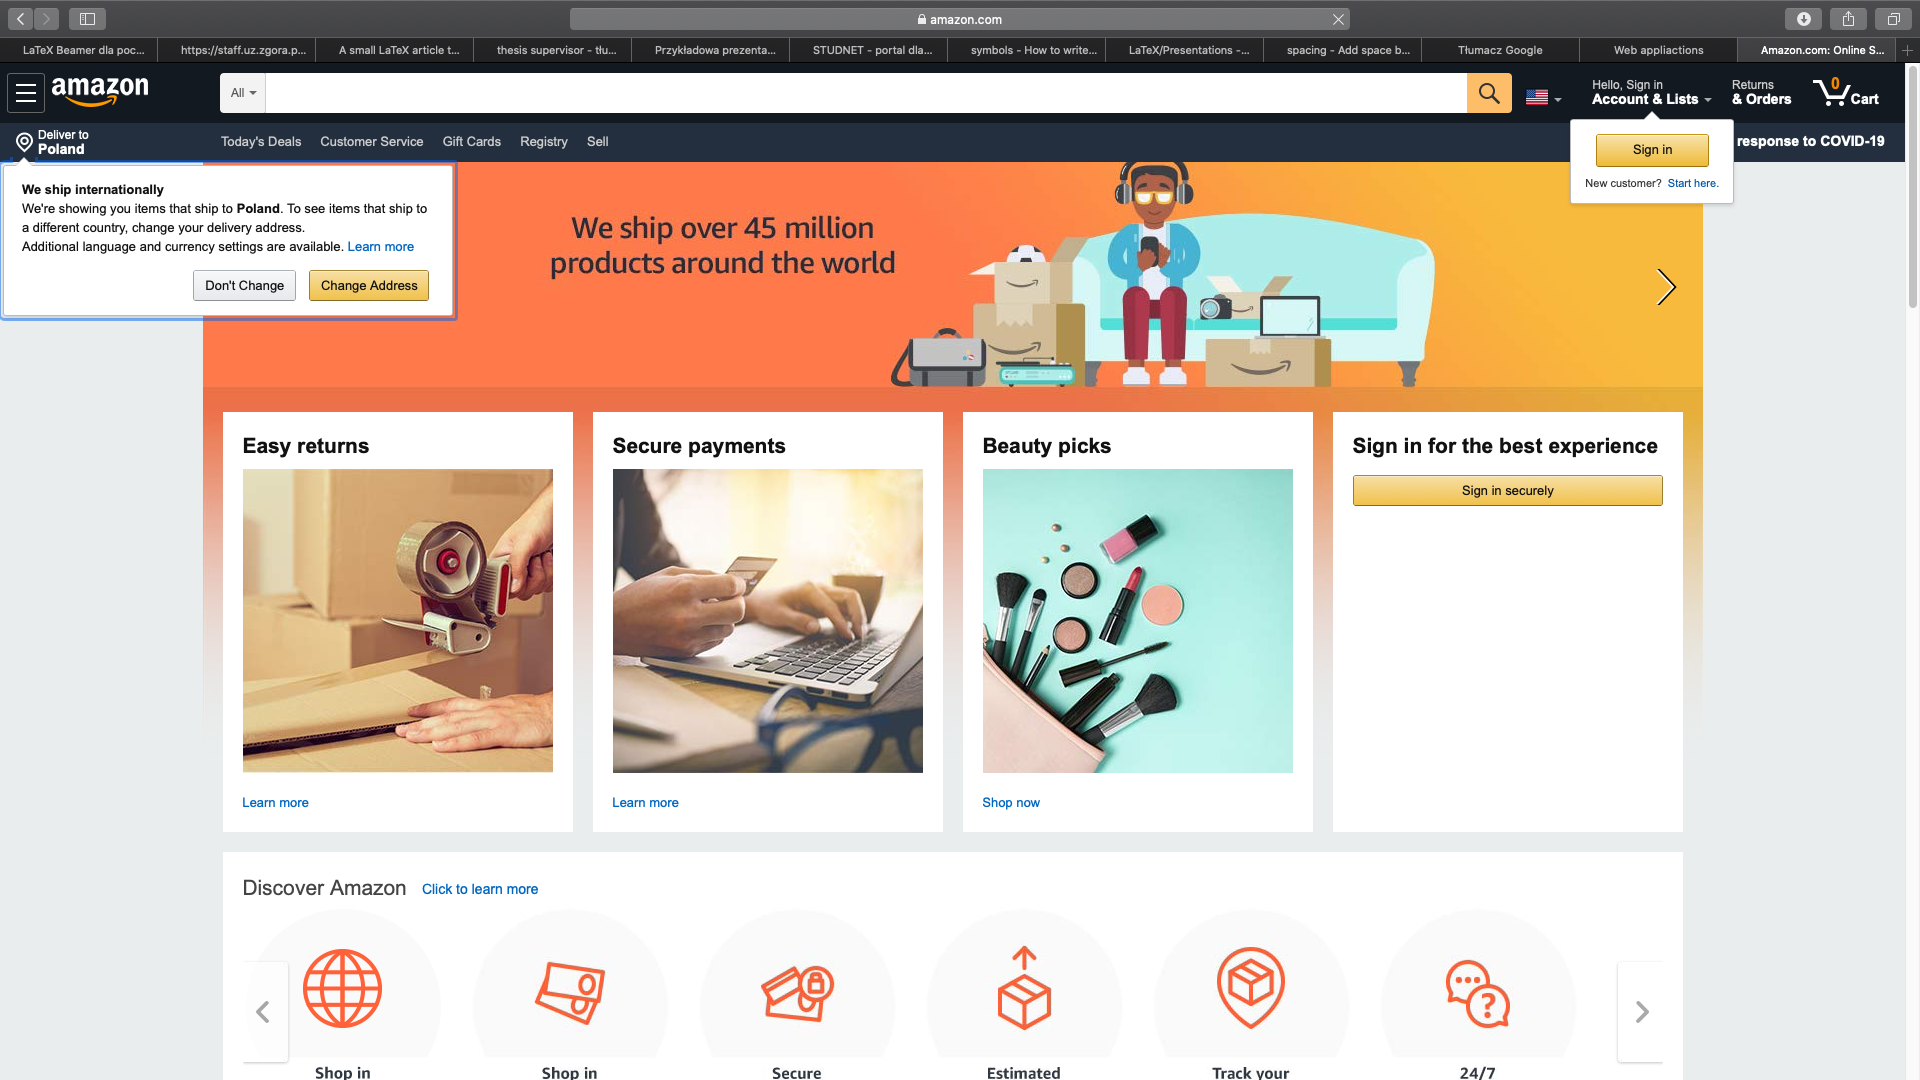
\includegraphics[width=\linewidth]{pictures/amazon}
    			\caption{Amazon}
  			\end{subfigure}
  			\begin{subfigure}[b]{0.3\linewidth}
    			
\includegraphics[width=\linewidth]{pictures/netflix}
    			\caption{Netflix}
  			\end{subfigure}
  		 	\begin{subfigure}[b]{0.3\linewidth}
    			
\includegraphics[width=\linewidth]{pictures/twitter}
    			\caption{Twitter}
  			\end{subfigure}
  				\caption{Examples of the modern web applications.}
  				\label{fig:coffee}
		\end{figure}
	\end{frame}
	
	\begin{frame}{Three-layer application model}
		Basic web applications have a presentation layer written using \textit{HTML}, as well as a program run on the server. Its task is service \textit{databases}, i.e. management of permanent data that is related to software
		
		\begin{itemize}
  			\item \textit{HTML} - markup language used for documents displayed in browser.
  			\item \textit{Database} - an application that stores and manages solid data.
		\end{itemize}
		
		\begin{figure}[h!]
			\centering
			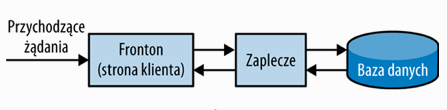
\includegraphics[height=2cm]{Pictures/architektura_trojwarstwowa}
			\caption{Three-layer application model scheme.}	
			\label{fig:architekturaTroj}
		\end{figure}

	\end{frame}
		
	\subsection{Mnolithic approach}
	\begin{frame}{Monolithic applications}
		\textbf{Monolith} means solid stone block. This sentence perfectly reflects the nature of this type of architecture. The application was written based on a three-layer model, except that the frontend and backend have a common code base. They are placed in a one repository and run with one executable file.
		\begin{figure}[h!]
			\centering
			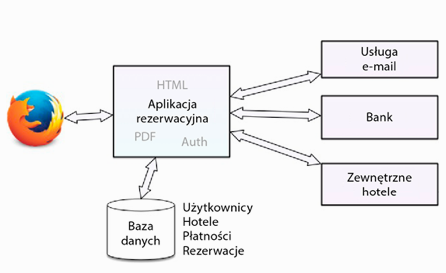
\includegraphics[height=4cm]{Pictures/scentralizowanaArchitektura.png}
			\caption{Scheme of the centralized service that book a hotel.}	
			\label{fig:mono}
		\end{figure}
	\end{frame}
	
	\begin{frame}{Architecture of the monolithic applications}
		Logical layers are commonly used to creat monolithic applications, that is why many techniques have been created to allow them to be organized. The most popular of them is the division of application layers into those that will be responsible for data access (Data Access Layer) by their management (Business Logic Layer) and user interactions (User Interace).
		\begin{figure}[h!]
			\centering
			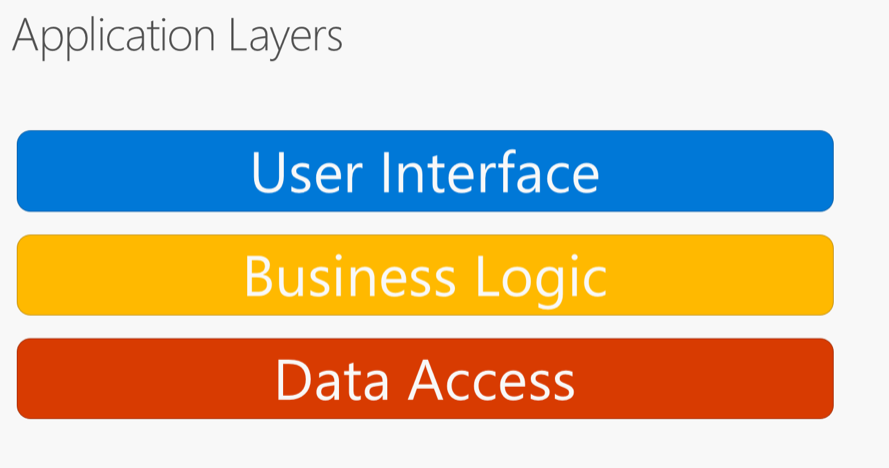
\includegraphics[height=3cm]{Pictures/warstwyAplikacji.png}
			\caption{Three-layer application architecture.}	
			\label{fig:architekturaTroj}
		\end{figure}
	\end{frame}
	
	\begin{frame}{Architecture of the monolithic applications}
		Modern frameworks further fragment the individual layers, to provide access only for programmers with interfaces that they can use to create their own application. \textit{Ruby on Rails} introduced \textit{MVC} and \textit{Django} \textit{MVT}.
		
		\begin{itemize}
  		\item \textit{MVC, (Model-View-Controller)} - where models are the classes responsible for interacting with the framework's database mechanism. Controllers, which task is to receive data from the user, modify the model and refresh views. The views, on the other hand, are responsible for generating HTML templates and sending them to the application client (user's browser).
  		\item \textit{MVT (Model-View-Template)} - Instead of using \textit{controllers}, that frameworks uses \textit{templates}. They do not differ much from the \textit{controllers}. Difference is that instead of classes generating HTML files, its creators have created a module responsible for processing such files with special tags. They provide additional logic to interact with the data sent through the view.
		\end{itemize}
	\end{frame}
	
	\subsection{Microservices}
	\begin{frame}{What are microservices?}
	An opposition to the approach where one central application communicates with external services is to create several smaller programs working separately. Their code could be divided into several separately run processes that have different smaller tasks to accomplish.
	
		\begin{figure}[h!]
			\centering
			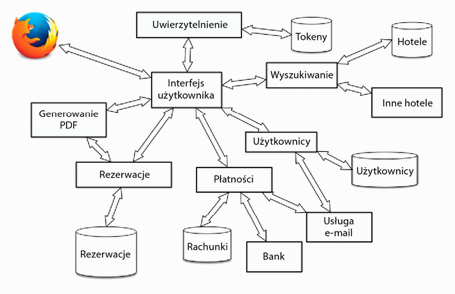
\includegraphics[height=4cm]{Pictures/mikrouslugi}
			\caption{Monolithic application from figure \ref{fig:mono} divided into microservices.}	
			\label{fig:architekturaTroj}
		\end{figure}
	\end{frame}
	
	\begin{frame}{Microservices architecture}
		There is no single template to determine the structure of the entire system based on microservices. Unlike monolithic applications, small independent websites do not require an in-depth design of the class hierarchy or relationships between individual modules. In this case, the most important is to look at the entire system from the side of messages, not from the perspective of individual components. It is then easier to analyze the ways of interaction between them, find the right patterns and adapt their architecture well. This point of view makes clear that for microservices, the most important thing is to design a transport layer. The knowledge that particular service is actually a separate HTTP server is very important.
	\end{frame}
	
	\section{Practical part}
	\subsection{Application project}
	\begin{frame}{Application project}
		\textbf{The goal:}
		\begin{itemize}
		  \item Create two separate application, the first one based on monolithic approach. The second one on microservices.
		  \item Implement database interactions for them.
		  \item Make usage of all HTTP response types.
		  \item Provide good communication layer for them.
		  \item Keep a similar technology stack for these applications.
		\end{itemize}
		\textbf{Technology stack:} \\
		\textit{Python, Flask, HTML, PostgresSql, Vue.JS}
	\end{frame}
	
	\begin{frame}{Database schema}
		The database will have two main tables: users and tasks. They will be connected by the one-to-many relationships in many frameworks also called a foreign key. This means that one user will be able to have many tasks assigned to each other, while one task will be assigned to only one user.
		\begin{figure}[h!]
			\centering
			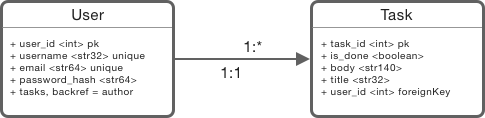
\includegraphics[height=2cm]{Pictures/databaseSchema}
			\caption{Application database schema.}	
			\label{fig:architekturaTroj}
		\end{figure}
	\end{frame}
	
	
	\begin{frame}{Architecures}
			\begin{figure}[h!]
			\centering
			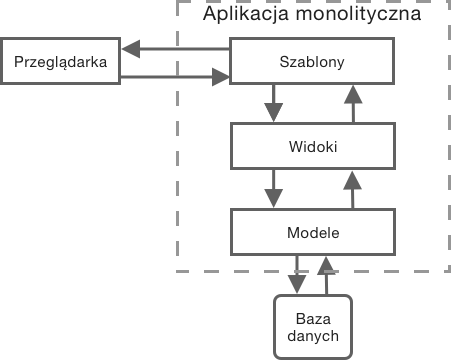
\includegraphics[height=2.7cm]{Pictures/architekturaMono}
			\caption{Monolithic application architecture schema.}	
			\label{fig:architekturaTroj}
		\end{figure}
		\begin{figure}[h!]
			\centering
			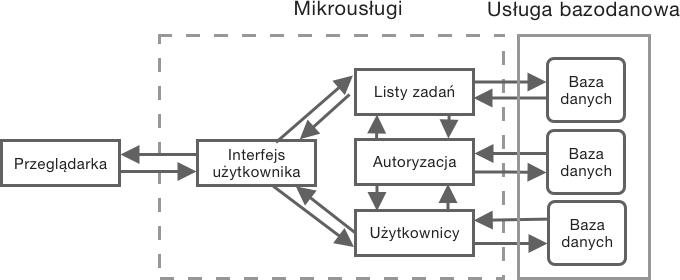
\includegraphics[height=2.3cm]{Pictures/architekturaMirko.png}
			\caption{Microservices application architecture schema.}	
			\label{fig:architekturaTroj}
		\end{figure}
	\end{frame}
	
	\subsection{Containerization}
	\begin{frame}{Integration with hosting services}
	Containerisation of the application with the Docker platform ensures the system's operation regardless of the programmer's machine, but it can also be used to create a production environment and integration with the server infrastructure. Services such as Amazon Web Services have ready solutions for publishing applications inside containers. \\
	~\\
	\textbf{Link to docker documentation:} \url{https://docs.docker.com}
	
	\begin{figure}[h!]
			\centering
			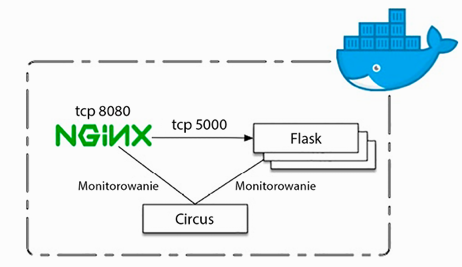
\includegraphics[height=3cm]{Pictures/docker}
			\caption{Example of the docker environment.}	
			\label{fig:architekturaTroj}
		\end{figure}
	\end{frame}
	
	\subsection{Application tests}
	\begin{frame}{Application tests}
		The studies in the thesis were about monolithic and microservices platforms performance, scalability and general opinion on writing applications and used technologies.\\
		~\\
		\textit{Boom} - program that was used to measure application performance. \url{https://github.com/tarekziade/boom} \\
		~\\
		\textbf{Test environment:}
		Machine with 2.7 GHz Intel Core i5 processor with RAM 8 GB 1867 MHz DDR3. \textit{Boom} in the configuration of 100 users who sent a maximum of 1000 requests.
	\end{frame}
	
	\subsection{Tests results}
	\begin{frame}{Endpoints performance}
		\begin{figure}[h!]
  			\centering
  			\begin{subfigure}[b]{0.45\linewidth}
    			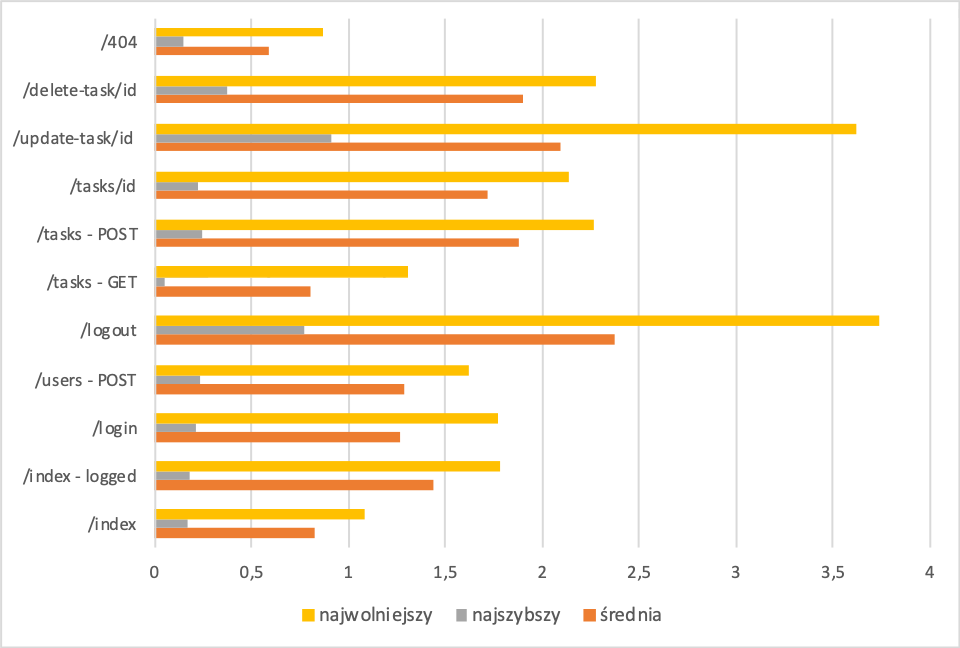
\includegraphics[width=\linewidth]{pictures/mono-zad}
    			\caption{Microservices}
  			\end{subfigure}
  			\begin{subfigure}[b]{0.45\linewidth}
    			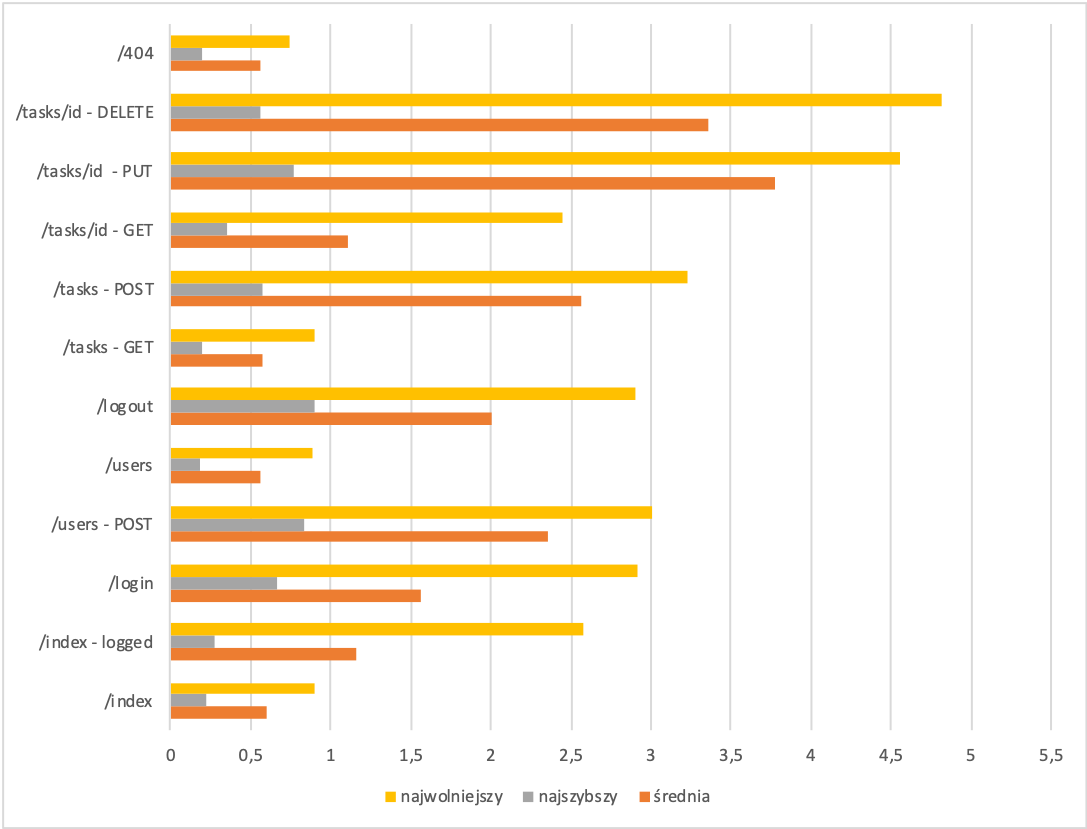
\includegraphics[width=\linewidth]{pictures/micro-zad}
    			\caption{Monolithic}
  			\end{subfigure}
  				\caption{Performance tests result response time(ms) foreach applications endpoint.}
  				\label{fig:coffee}
		\end{figure}
	\end{frame}
	
	
	\begin{frame}{Vertical scalability performance tests}
		\begin{figure}[h!]
  			\centering
  			\begin{subfigure}[b]{0.45\linewidth}
    			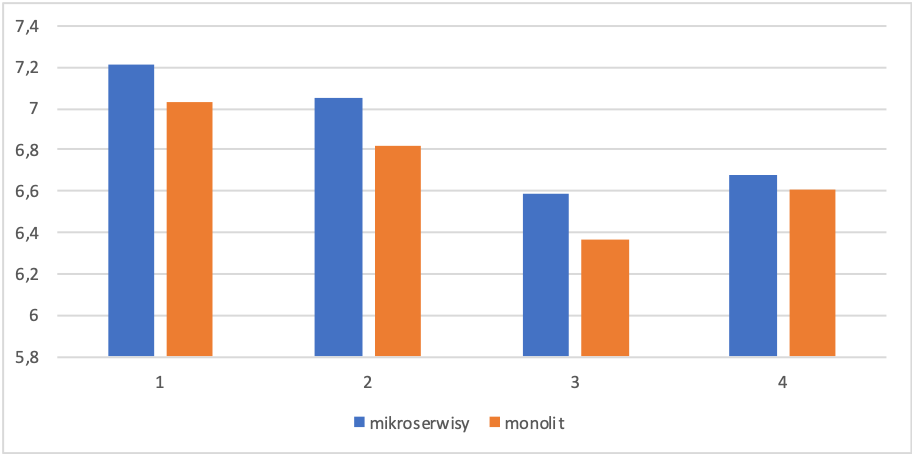
\includegraphics[width=\linewidth]{pictures/cputest}
    			\caption{Request average time(ms) for amount of CPU cores (GHz).}
  			\end{subfigure}
  			\begin{subfigure}[b]{0.45\linewidth}
    			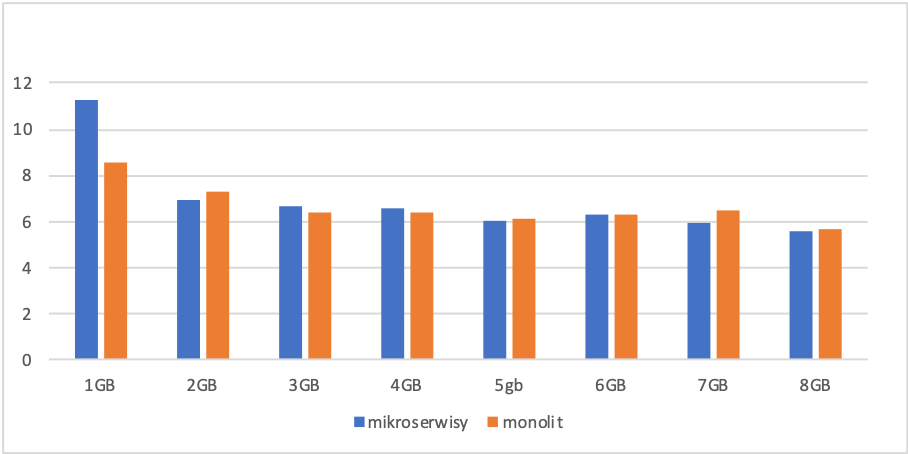
\includegraphics[width=\linewidth]{pictures/ramtest}
    			\caption{Request average time(ms) for amount of RAM(Gb).}
  			\end{subfigure}
  				\caption{Performance tests result for vertical scalability (RAM and CPU tests).}
  				\label{fig:coffee}
		\end{figure}
	\end{frame}
	
	\begin{frame}{Horizontal scalability performance tests}
		\begin{figure}[h!]
			\centering
			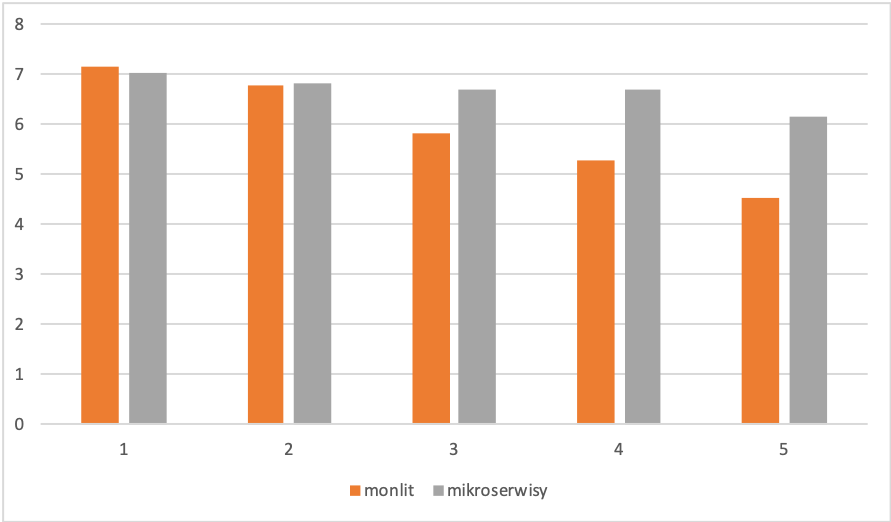
\includegraphics[height=5cm]{Pictures/kontenery}
			\caption{Request average time(ms) for amount of the containers for each service.}	
			\label{fig:architekturaTroj}
		\end{figure}
	\end{frame}
	
	\subsection{Conclusions}
	\begin{frame}{Conclusions}
	The conducted research indicates better performance of the monolithic website, but it should be noted that the created application is small, the HTML templates generated by it were small. Microservices, despite the fact that they send only JSON objects, still have to be serialized, which could burden the application without highlighting the advantages of this solution. In addition, the services would be launched inside containers, which, despite the fact that they can be used in production solutions, require more resources. Running more containers in a decentralized application could also affect their response times. Another factor that could affect the research was the hardware limitations of the physical machine. It was not a unit prepared exclusively for server solutions and it had a limited number of RAM, an older generation processor and a small disk space.
	\end{frame}
	
	\section{Summary}
	\begin{frame}{Conclusions}
	Finally, one can come to the conclusion that the choice between monolithic architecture and microservices should be directed mainly due to the nature of the web application project. When it comes to created as part of a larger team that knows several technologies, it would be reasonable to divide the application so that each of them works on a separate service, then for larger services, it will be possible that the disadvantages of a solution based on microservices will be less significant.
	
	 A monolithic application is still a good idea for smaller applications, where the team does not consist of a large number of people familiar with several technologies. Starting a project is then much simpler and the implementation of such an application is faster. In the event that it grows to a larger size, there is an option to rewrite it to a smaller application and change the architecture to that based on microservices.	
	\end{frame}

	
	\section{Figure sources}
	\begin{frame}{Figure source}
		\begin{itemize}
  			\item Figure 1: screens of the main pages: \textit{Amazon} (\url{https://amazon.com}), \textit{Netflix} (\url{https://netflix.com}), \textit{Twitter} (\url{https://twitter.com})
  			\item Figure 2: source: Tarek Ziadé. Rozwijanie mikrousług w Pythonie. Budowa, testowanie, instalacja i skalowanie. Helion, 2018.
  			\item Figure 3, 5: source: Susan J. Fowler. Mikrousługi. Wdrażanie i standaryzacja systemów w organizacji inżynierskiej. Helion, 2019.
  			\item Figure 4:  © Microsoft 2020. Dokumentacja Microsoft Build. https://docs.microsoft.com/pl-pl/.
		\end{itemize}
		
		\textit{The rest of the figures is the author's own study.}
	\end{frame}
	
	\begin{frame}[allowframebreaks]
		\frametitle{References}
	    \begin{itemize}
 			\item Tarek Ziadé. Rozwijanie mikrousług w Pythonie. Budowa, testowanie, instalacja i skalowanie. Helion, 2018.
 			\item Susan J. Fowler. Mikrousługi. Wdrażanie i standaryzacja systemów w organizacji inżynierskiej. Helion, 2019.
 			\item Richard Rodger. Tao Mikrousług. Projektowanie i wdrażanie. Helion, 2019.
 			\item Sam Newman. Budowanie mikrousług. Helion, 2019
 			\item Daniel Nations. What exactly is a web application? Lifewire, 2019. https://www.lifewire.com/what-is-a-web-application-3486637.
 			\item  © Microsoft 2020. Dokumentacja Microsoft Build. https://docs.microsoft.com/pl-pl/.
 			\item "Ruby on Rails" David Heinemeier Hansson. All rights reserved "Rails". Dokumentacja Ruby on Rails. https://guides.rubyonrails.org.
 			\item © 2005-2020 Django Software Foundation and individual contributors. Dokumentacja Django w wersji 3.0. https://docs.djangoproject.com/en/3.0/.
 			\item © Copyright 2010 Pallets. Dokumentacja Flaska w wersji 1.1.x. https://flask.palletsprojects.com/en/1.1.x/.
 			\item Copyright © 2014-2020 Evan You. Dokumentacja Vue.JS w wersji 2.x. https://vuejs.org/v2/guide/.
 			\item Copyright © 2013-2020 Docker Inc. Dokumentacja Dockera. https://docs.docker.com/.
		\end{itemize}
	\end{frame}
\end{document}
